\chapter{Modeling}
The objective of this thesis is the grouping of expenses with the methods of \ac{NLP}. Grouping, or clustering, is the practise of sorting data points into groups in such a way that the similarity inside a group (intra-cluster similarity) is high while the similarity between clusters (inter-cluster similarity) is low. The defintion of similarity as well as different clustering algorithms are presented and contrasted in the following sections.


\section{Alternatives}
\subsection{Similarity and distance measures}
A distance measure is a quantification of how near objects in space are. Distance measures can be defined for spaces of arbitrary numbers of dimensions. In the examples, four words (man, woman, king, queen) are compared in their semantic similarity. The word vectors were generated with a word embedding, but the focus is on comparing the distance measures available for clustering later on.

		\begin{figure}[!h]
			\centering
			\includegraphics[height=6cm]{Bilder/models/heatmap_dot_product.pdf}
			\caption{Dot Product as Similarity Measure}
			\label{fig:dotproduct-heatmap}
		\end{figure}
	
		\subparagraph{Dot Product}
		The dot product is an operation transforming a vector into a scalar through multiplying the vectors element-wise. This operation is easily and efficiently calculated, but has some pitfalls.
		While every word in the example (\ref{fig:dotproduct-heatmap}) ranks very high in similarity to itself, the distance between the word and itself is not always the same for every word. This happens because the dot product is not agnostic of a vector's magnitude. A vector's product with itself is the square of its magnitude. This results in the similarity of man-man to be lower than the similarity of queen-queen.
		This fact makes the dot product impractical for accurately representing the relationships of words.
	
					\[ 
				\text{dot product} :=  \mathbf{A} \cdot \mathbf{B}= \sum\limits_{i=1}^{n}{A_i  \mathbf{B}_i} 
				\]

	
		\subparagraph{Euclidean Distance} \label{euclidean}
		For low-dimensional applications, this distance works well and shows great results. Euclidean distance can be calculated in a highly efficient manner, even for n dimensions. This suggests, that euclidean distance is particularly suitable for high-dimensional data. Unfortunately, euclidean distance falls victim to the curse of dimensionality. In \cite[p.~1]{beyerNearestNeighbor} it is proven that with increasing dimensions, the distance between data points approaches an uniform value for all data points. This effect could be demonstrated for spaces with as little as ten dimensions. Therefore, it can be said that euclidean distance is not suitable for high-dimensional data. With vectors in \ac{NLP} ranging from 100 to 800 dimensions with embeddings and hundreds of thousands with \ac{TF-IDF}, this distance measure is not suitable.
		
				\[ 
		\text{euclidean distance} :=  \sum\limits_{i=1}^{n}{(A_i -  \mathbf{B}_i)^{2}} 
		\]
		
		\begin{figure} 
			\begin{minipage}{0.49\textwidth}
				\label{fig:euclidean}
				
				\includegraphics[height=5cm]{Bilder/models/euclidean}
				\caption{Euclidean Distance as Measure}
			\end{minipage}
			\hfill
			\begin{minipage}{0.49\textwidth}
				\includegraphics[height=5cm]{Bilder/models/cosine}
				\caption{Cosine Similarity as Measure}
				\label{fig:cosine}
			\end{minipage}
			\hfill
		\end{figure} 
	
		\subparagraph{Cosine Similarity}
		The name of this measure already suggests that not distance but similarity of objects is measured. Instead, it quantifies how close two vectors are.  Mathematically, the cosine distance is the cosine of the angle between two vectors. A wide angle means a high distance between two vectors, or in this case two words. Narrow angles stand for a low distance and words being closely related. In example \ref{fig:cosine}, the word vectors for woman and king have a higher angle than those of woman and queen. This means the words woman and queen are more similar thank woman and king.
		
		\[ 
		\text{cosine similarity} := \cos(\theta) = {\mathbf{A} \cdot \mathbf{B} \over \|\mathbf{A}\| \|\mathbf{B}\|} = \frac{ \sum\limits_{i=1}^{n}{\mathbf{A}_i  \mathbf{B}_i} }{ \sqrt{\sum\limits_{i=1}^{n}{\mathbf{A}_i^2}}  \sqrt{\sum\limits_{i=1}^{n}{\mathbf{B}_i^2}} }
		  \]
		
		The difference between cosine distance and euclidean distance is clear: cosine measures the angle, and euclidean the vector length. But which one performs better in high dimensions? Cosine distance is perceived as more suitable for high dimensional data \cite[c.2.1.2.1]{40algorithms}, and often suggested for \ac{NLP} tasks. 
		
		But there is one fact left out in this suggestion: On normalized data (all vectors are unit vectors), cosine distance and euclidean distance are linearly connected \cite{khanRelationshipCosineSimilarity2020}.
		
		\begin{align*}
			\cos(\theta_{AB}) &= {\mathbf{A} \cdot \mathbf{B} \over \|\mathbf{A}\| \|\mathbf{B}\|}  \\
			\\
			\text{for normalized vectors with } \|\mathbf{A}\| &=1 \text{ and } \|\mathbf{B}\| =1: \\
			\cos(\theta_{AB}) &=  {\mathbf{A} \cdot \mathbf{B} \over 1 * 1 } = \mathbf{A} \cdot \mathbf{B}
		\end{align*}
		
		\begin{align*}
			d(\mathbf{A}, \mathbf{B}) &:=  \sum\limits_{i=1}^{n}{(\mathbf{A}_i -  \mathbf{B}_i)^{2}} \\
			&= \sum\limits_{i=1}^{n}{\mathbf{A}_i^{2} - 2\mathbf{A}_i\mathbf{B}_i + \mathbf{B}_i^2}  \\ 
			&= \sum\limits_{i=1}^{n}{\mathbf{A}_i^{2}} + \sum\limits_{i=1}^{n}{- 2\mathbf{A}_i\mathbf{B}_i} + \sum\limits_{i=1}^{n}{\mathbf{B}_i^2} \\
			&= 	\|\mathbf{A}\| + \sum\limits_{i=1}^{n}{- 2\mathbf{A}_i\mathbf{B}_i} + \|\mathbf{B}\| \\
			&= \|\mathbf{A}\| -2 \sum\limits_{i=1}^{n}{\mathbf{A}_i\mathbf{B}_i} + \|\mathbf{B}\| \\
			&= \|\mathbf{A}\| -2 (\mathbf{A} \cdot \mathbf{B}) + \|\mathbf{B}\| \\
			\\
			\text{for normalized vectors with }\|\mathbf{A}\| &=1 \text{ and } \|\mathbf{B}\| =1  \text{ and } \mathbf{A} \cdot \mathbf{B}  = \cos(\theta_{AB}):\\
			d(\mathbf{A}, \mathbf{B}) &= 1 - 2 \cos(\theta_{AB}) + 1 = 2 - 2(\cos(\theta_{AB})) \\
			\\
			\text{Both solutions are linear to ea}& \text{ch other:} \\
			2 - 2(\cos(\theta_{AB})) &\sim \cos(\theta_{AB})
		\end{align*}
	
		Now, with the newly gained insight into the distance relationships of normalized vectors of $\cos(\theta_{AB}) = \mathbf{A} \cdot \mathbf{B}$ and $d(\mathbf{A}, \mathbf{B}) = 2 - 2(\cos(\theta_{AB}))$ , it can be stated that the cosine distance and euclidean distance of two normalized vectors are linearly related.
				
		Cosine and euclidean distance being connected linearly for normalized data has not made the decision easier. But there is an additional factor: 
		Algorithms often require distance metrics to obey the four requirements of a metric space \cite{schubertTriangleInequalityCosine2021}.
		These requirements are \cite{rajaramanNeighborSearchHigh}:
		\begin{enumerate}
			\item The distance between to points is 0 if and only if they are identical.
			\item The distance between two points is never negative.
			\item The distance is equal irrespective of the starting point.
			\item The shortest distance between two points is a straight line.
		\end{enumerate} 
		
		All aforementioned arguments make a strong case for the euclidean distance.
		
\subsection{Clustering Algorithms}
		
		\subparagraph{K-Means}
		The k-Means algorithm generates $k$ groups of data by iteratively adapting clusters and their centers. The algorithm is mainly focused on performance, hence the design is kept lean by omitting logic for determining the number of clusters \cite[c.6.2]{40algorithms}. Following pseudo code illustrates the workings of the algorithm.
		
		\begin{lstlisting}
randomly choose k_centers
while (iterations < max_iterations):
	assign each point to nearest center in k_centers
	mean of each cluster's elements are k_centers_new
	if k_centers == k_centers_new:
		break
		\end{lstlisting}
	
			 \begin{figure}[!h]
		\centering
		\includegraphics[height=15cm, angle=90]{Bilder/models/minibkmeans.pdf}
		\caption{How MiniBatchKmeans recognizes Clusters \cite{sklearn}}
		\label{fig:kmeans-viz}
		\end{figure}
	
		The k-Means algorithm performs reasonably well in identifying clusters in data such as in figure \ref{fig:kmeans-viz}. The left example seems unspectacular, but in the center example, it becomes obvious that k-Means is prone to overfit on noisy data. This can be partially blamed on the focus on centers, and not density. The focus on centers is also obvious in the rightmost example. While the data is quite evenly distributed over the area, the algorithm still groups the data. 
		
		Implementations such as \ac{sklearn}'s \lstinline|MiniBatchKMeans| \cite{sklearn} speed up the computation time by processing subsets of the data in a parallel way. While only achieving almost perfect results \cite{sculleyWebscaleKmeansClustering2010}, the batched k-Means algorithm is of special appeal when handling large data sets.
		
		This algorithm has the advantage of high performance, and performs well on large data sets. Unfortunately, the quality of the results depend highly on choosing the correct parameters. Also, k-Means is not robust against outliers, and results are not reproducible since the first cluster centers are chosen randomly \cite[c.6.2]{40algorithms}.
		
		\subparagraph{\acl{DBSCAN}}
		The \ac{DBSCAN} clustering algorithm was developed to solve the problem of needing domain knowledge while tuning cluster models \cite{DBSCAN}. The algorithm uses an intuitive approach for identifying which points belong into a cluster, and which are outliers.

		For two points to be considered neighboring (density-reachable, \cite{DBSCAN}), they have to be within a certain distance to each other: \lstinline|eps|. Neighboring points are categorized into one cluster, expanding the reach of this cluster over all values within the distance \lstinline|eps|.
		But, there is a limitation to the points being able to expand a cluster. If the cluster were to expand without limitations apart from a maximum distance, the clusters would be able to "spread" from one cluster to another if connected by one data point.
		To prevent this, only center points can expand the cluster. A center point has a minimum number of neighboring points (\lstinline|min_samples|). This helps to create dense clusters and prevents the undesirable spreading.
		
		 \begin{figure}[!h]
			\centering
			\includegraphics[height=15cm, angle=90]{Bilder/models/dbscan.pdf}
			\caption{How DBSCAN recognized Clusters and Outliers \cite{sklearn}}
			\label{fig:dbscan-viz}
		\end{figure}
	
		Figure \ref{fig:dbscan-viz} illustrates how \ac{DBSCAN} does not fall prey to outliers, as k-Means does. A broad distribution of data points in the left example is very intuitively grouped into clusters and outliers. Especially the center picture showcases the ability of DBSCAN to recognize clusters by their density. The even spread of data in the third example is also correctly identfied as one large cluster, even though a small part of the data was not within \lstinline|eps| range.
		
		But areas of high density do not say anything about being topically related.

		
\subsection{Topic Model}
After documents are clustered, each cluster needs a meaningful label to provide actual value. This task is called topic modeling. Several methods exist for generating or extracting labels from clustered data. 

Firstly, the word frequency in one cluster can determine the topic. Each word is evaluated with respect to its frequency over the whole cluster. Either the most frequent one or top n words can be the topic.
This method is quite prone to skewing by one document containing a word many times.

The second method uses the document frequency. This measure is also part of the \ac{TF-IDF} measure (\ref{section:tfidf}).
The \ac{TF-IDF} vectorization method had to basic assumptions:
\begin{enumerate}
	\item Words with a high frequency in a document describe it well.
	\item Words with a high frequency in a corpus do not describe one specific document well.
\end{enumerate}

But the second assumption does not hold true any more when applied to a cluster. Clusters should already be very similar, and contain similar words. Therefore, words occurring often over many different documents describe the cluster very well. The metric for this is the document frequency:

\[ DF(t_{i}) =\dfrac{\#(d_{t_{i}}) }{|C|} = \dfrac{ number \; of \; documents \; containing \; word \; t_{i}}{number \;  of\;  documents \;  in \; cluster \; C} \]

The document frequency of a word is the relative share of documents in the cluster it occurs in.

\subsection{Dimensionality Reduction}

The embeddings generated in the data preparation section are 512-dimensional. While the clustering algorithms work well with processing this data, 512 dimensions are not imaginable with the human mind. To visualize clusters, these dimensions have to be projected onto a two-dimensional plane. This task is called \ac{DR}, and is unsupervised. 

Selecting a \ac{DR} method, there are important aspects to consider:
\begin{itemize}
	\item How well can the algorithm preserve the distances in the clusters (local structure)?
	\item How well can the algorithm preserve the distances between the clusters (global structure)?
\end{itemize}

Data scientists have many methods for \ac{DR} at hand, some of the most popular ones being \ac{t-SNE} and \ac{PCA}.

The \ac{PCA} identifies principal components in the dataset with an unsupervised \ac{ML} algorithm.\cite{40algorithms} A principal component is an axis in the multidimensional space along which the variance is maximized \cite{pcaVStsne}. The number of learned principal components depends on the number of target dimensions, in the case of visualizations either two or three dimensions and principal components. The principal components are orthogonal to each other and span the hyperplane on which the values are projected \cite{pcaVStsne}.
It is important to note that \ac{PCA} approximates the values, trading in accuracy for performance \cite{40algorithms}.

\ac{t-SNE} is focused on retaining as much structure, both globally and locally. It does so by computing pairwise similarities in the dataset. The algorithm uses these similarities to accurately represent the same distances in a lower number of dimensions. This design of \ac{t-SNE} helps to represent existing clusters very well.

The two methods are contrasted on the task of representing three-dimensional clusters (Figure \ref{fig:original}) in two dimensions. This task is quite similar to the later application of the \ac{DR} algorithm. In figure \ref{fig:pca} the \ac{PCA} algorithm proves that it is able to represent the global structure in some way, but not quite satisfactory. It is heavily outperformed by \ac{t-SNE}, in both preserving the global distances and the local structures. Apart from two clusters merging, the algorithm forms very distinct and clean clusters.

Overall, design and the practical application of the \ac{t-SNE} algorithm make the case for it.




\begin{figure} 
	\begin{minipage}{0.3\textwidth}
		
		\includegraphics[width=\textwidth]{Bilder/models/original.pdf}
		\captionsetup{labelformat=empty}
		\centering
		Original 3D Clusters
		\label{fig:original}
	%	\caption{Original 3D Clusters}
	%	\addtocounter{figure}{-1}
	\end{minipage}
	\hfill
	\begin{minipage}{0.3\textwidth}
		
		\includegraphics[width=\textwidth]{Bilder/models/pca.pdf}
		\label{fig:pca}
		\captionsetup{labelformat=empty}
		\centering
		\ac{PCA}
	%	\caption{\ac{PCA}}
	%	\addtocounter{figure}{-1}
	\end{minipage}
	\hfill
	\begin{minipage}{0.3\textwidth}
		
		\includegraphics[width=\textwidth]{Bilder/models/tsne.pdf}
		\label{fig:tsne}
		\captionsetup{labelformat=empty}
		\centering
		\ac{t-SNE}
	%	\caption{\ac{t-SNE}}
	%	\addtocounter{figure}{-1}
	\end{minipage}
\caption{Dimensionality Reduction on three-dimensional Clusters}
\end{figure} 

\section{Theoretical Implementation}

\begin{table}[!h]

	\begin{tabular}{lll}
		\textbf{Task}            & \textbf{Alternatives}                                                                      & \textbf{Planned Implementation}                                                               \\
		Distance Measure         & \begin{tabular}[c]{@{}l@{}}Dot Product\\ Euclidean Distance\\ Cosine Distance\end{tabular} & Euclidean Distance                                                                               \\
		Clustering               & \begin{tabular}[c]{@{}l@{}}k-Means\\ DBSCAN\end{tabular}                                   & \begin{tabular}[c]{@{}l@{}}DBSCAN for outlier detection\\ k-Means for clustering\end{tabular} \\
		Topic Modeling           & \begin{tabular}[c]{@{}l@{}}Word Frequency\\ Document Frequency\end{tabular}                & Document Frequency                                                                            \\
		Dimensionality Reduction & \begin{tabular}[c]{@{}l@{}}PCA\\ t-SNE\end{tabular}                                        & t-SNE                                                                                        
	
	\end{tabular}
	\caption{Tasks during the Modeling Phase}
	 \label{table:modeling}
\end{table}


The table \ref{table:modeling} sums up all available alternatives from the prior section and the chosen alternative. The implementation of the modeling part starts with an analysis of the cosine distances in the dataset. For this, the KNeighbors algorithm will show the distance of each datapoint to its next neighbor. Next the outliers are sorted out with the DBSCAN clustering method. Before training the k-Means model, the ideal number of clusters has to be found with the elbow method. The k-Means model identifies the clusters. Topics per cluster are generated and the clusters are visualized with t-SNE.



\section{Practical Implementation}

\subsection{Determining composition of dataset with KNeighbors Algorithm}


Both density-based and distance-based clustering algorithms work with distances between objects. Before any clustering is applied, an overview over the distances should be established \cite{maklinDBSCANPythonExample2022a}. This allows to make meaningful decisions while hyperparameter-tuning.

 \begin{figure}[!h]
	\centering
	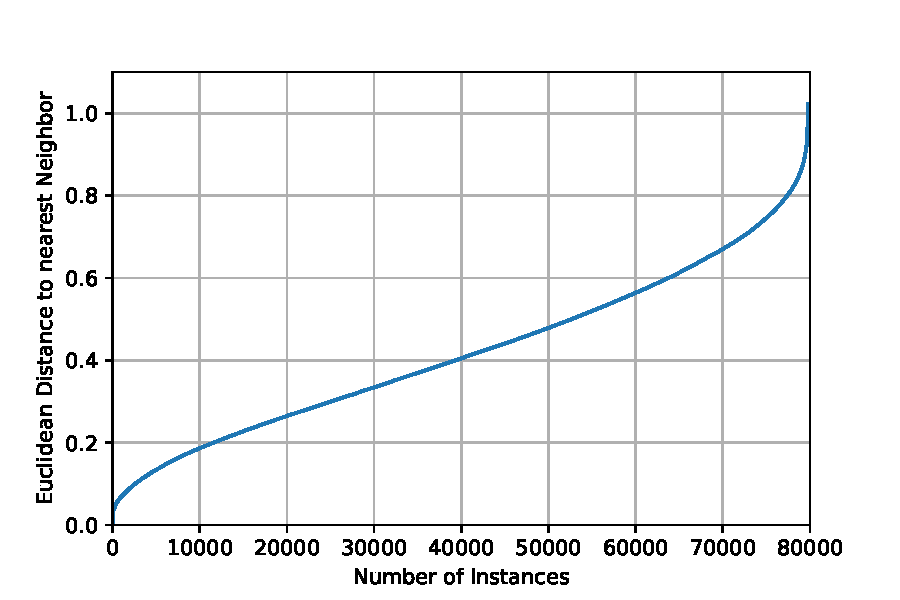
\includegraphics[height=8cm]{Bilder/models/kneighbors.pdf}
	\caption{Each Instance's Distance to the nearest neighboring Point}
	\label{fig:dbscan-plot}
\end{figure}

This can be done with the algorithm \lstinline|sklearn.neighbors.NearestNeighbors|, which takes the input of a dataset with arbitrary dimensions. Using a specified distance metric, the algorithm outputs the distance of each data point to its nearest neighbor in the data set. The distance metric used is the euclidean distance.
The distance search shows that almost all points are within a maximum distance of 0.8 to the next neighbor. All other points are outliers and will be filtered out with \ac{DBSCAN}.



\subsection{Preselect documents with \ac{DBSCAN}}
The \ac{DBSCAN} algorithm outputs, apart from clusters, outlier data points which do not belong into any cluster. With this algorithm, outliers in the data are detected to prevent the main clustering algorithm (KMeans) from overfitting. 
The clustering algorithm has the parameters \lstinline|eps| and \lstinline|metric| which tune the model.

The (distance) \lstinline|metric| is of course cosine. The \lstinline|eps| stands for the maximal distance between two points to be considered a neighbor \cite{SklearnClusterDBSCAN}. As established before, the outliers are those points which are more than 0.4 units separated from the next data point. Therefore, \lstinline|eps| is set to 0.4. 

The \ac{DBSCAN} model identified the outlier data (\ref{fig:dbscan-outliers}), amounting to about 3\% of the data points. These data points are not included into clustering by k-Means.

\subsection{Determine the number of Clusters}
The KMeans algorithm is parameterized with the number of clusters (\lstinline|n_clusters|). Since the algorithm itself is not able to determine the cluster count, this number has to be approximated.
\cite{kodinariyaReviewDeterminingCluster2013} suggest several applicable methods, among them are rule of thumb, and the elbow method with a silhouette score.
A good point for starting with choosing \lstinline|k| is the rule of thumb $k \approx \sqrt{\frac{n}{2}}$ with n being the number of instances in the dataset. Other literature also names the approximation of $k \approx log(n)$, but \cite{maierOptimalConstructionKnearest2009} showcase how $k$ should be chosen in the order of $n$. 

\begin{table}[!h]
	\centering
	
	\begin{tabular}{l|ll}
		\toprule
		heuristic for best k                         & k &  \\
		\midrule
		$k \approx \sqrt{\frac{n}{2}}$ &  199 &  \\
		$k \approx log(n)$             & 12   &  \\
		$k \approx n$                  &  e.g. 10 000, 20 000& 
	\end{tabular}
\caption{Three possible estimates for the optimal $k$}
\label{table:heuristic-k}
\end{table}

With the elbow method, the silhouette score of clustering results for different values of \lstinline|k| are visualized. 

The silhouette score is a measure of how similar intra-cluster points are and at the same time how dissimilar inter-cluster points are. A silhouette score of 1, being the highest value, is the most desirable.

The silhouette score $s$ of each data point $i$ can be calculated with the following formula \cite{kodinariyaReviewDeterminingCluster2013}:
\[ s(i) = \frac{b(i) - a(i)}{\max\{a(i),b(i)\}} \]

The measure $a$ denotes the mean distance to other points in the same cluster as $i$. This is interpreted as the inter-cluster dissimilarity, the higher $a(i)$, the more $i$ doesn't belong into the cluster.

The measure $b$ stands for the mean distance between $i$ and the points in the nearest other cluster. To identify the nearest other cluster to the point $i$, all mean distances to points of each cluster are calculated. The cluster with the smallest mean distance between all its points and $i$ is the neighboring cluster. The measure $b$ is interpreted as the similarity of $i$ to other clusters.

Being calculated for every point, this measure always falls in the interval $[-1;1]$. For $S = 1$, the relationship of $a(i)$ and $b(i)$ has to be $a(i) \ll b(i)$ so that the denominator and divisor each tend to $b(i)$ resulting in $S = 1$. This would mean that the point $i$ would have to be very far away from points in other clusters and very near to its own cluster. The value $S = 1$ is therefore the most desirable.

For $S = 1$, the relationship of $a(i)$ and $b(i)$ has to be $a(i) \gg b(i)$ so that the denominator and divisor each tend to $-a(i)$ respective $a(i)$ resulting in $S = -1$. In distance terms this means that the point $i$ is very far away from its own cluster points and very close to points in the next nearest cluster.

Therefore, the task of the elbow method using the silhouette coefficient is to maximize $S$ while preventing overfitting.

The above mentioned estimates (\ref{table:heuristic-k}) are a starting point for choosing values for k during the calculation of silhouette coefficients. The following simulation shows how the k-Means algorithm for these values of k performed.

 \begin{figure}[!h]
	\centering
	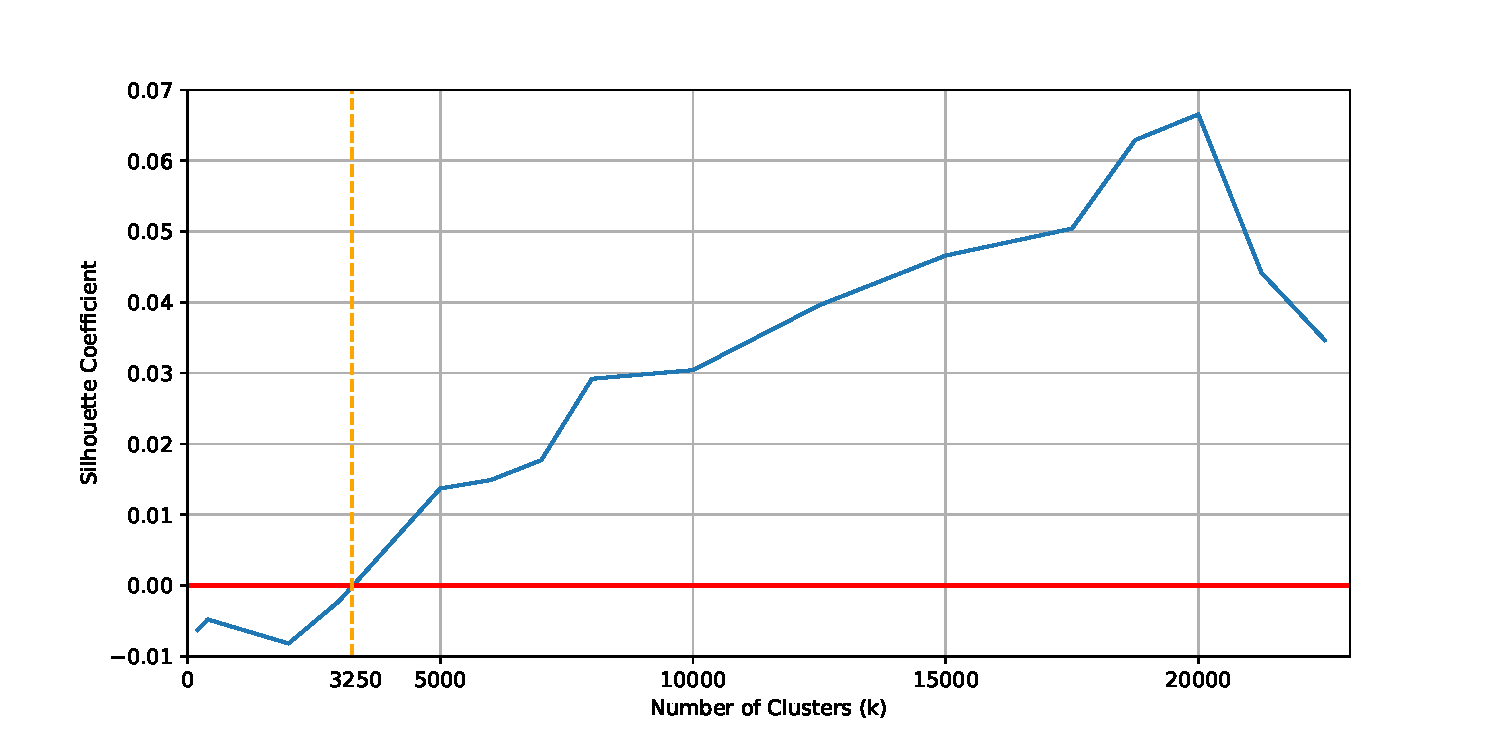
\includegraphics[height=8.5cm]{Bilder/models/elbow.pdf}
	\caption{Each Instance's Distance to the nearest neighboring Point}
	\label{fig:silhouette}
\end{figure}

The chart \ref{fig:silhouette} shows how the silhouette coefficient behaves with respect to k-Means models with different numbers of clusters. The x-axis shows the number of clusters, which the algorithm was configured with. The diagram was created by executing several runs of \lstinline|MiniBatchKMeans|. In the used dataset, the DBSCAN algorithm already filtered out the outliers.

The chart shows how the silhouette coefficient falls under the 0 threshhold. A negative silhouette coefficient means that points in one cluster were misclassified as they are more close to other clusters. This is an indicator of underfitting. 

But not only the left hand side of the spectrum for k can cause problems. When increasing k, the silhouette coefficient rises. In fact, one could obtain a perfect silhouette coefficient of 1 by assigning each point its own cluster \cite{yildirimTwoChallengesKMeans2020}. But with rising number of clusters, the generalization becomes lower. Again, the goal is a useful generalization. And dividing a group of 79741 documents into 20.000 groups can not be considered a useful generalization.

So, even though the silhouette method is very helpful as a technical analysis, the business goals have to be kept in mind. The silhouette coefficient at 0 means that on average, no points were misclassified due to underfitting. This minimal requirement is satisfied with $k$=3250.

\subsection{Train a KMeans Model}

The training with k=3250 takes about four minutes. Most clusters formed are in the size of 10 to 50 documents. The largest cluster contains 395 samples.

\begin{figure}[!h]
	\centering
	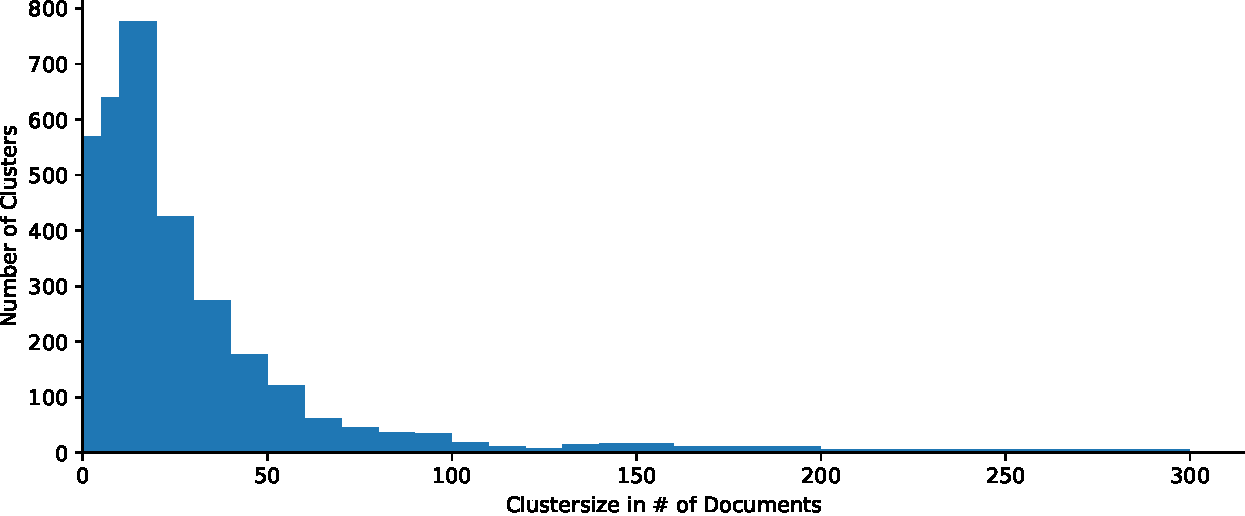
\includegraphics[height=6.5cm]{Bilder/models/clustersize.pdf}
	\caption{Distribution of the Cluster Sizes}
	\label{fig:clustersize}
\end{figure}

\subsection{Visualize cluster formation}
For visualizing, the \ac{t-SNE} algorithm is used. This projection allows to visualize the 512 dimensions of the embeddings in a two-dimensional representation. In figure \ref{fig:kmeans}, the proximity of points stands for their close semantic relationship. Data points in the same color are contained in the same cluster. Since there are 3250 clusters, colors occur several times, even though they represent different clusters.

This visualization gives an overview on the clusters, but doesn't show what is contained in the clusters. For this, each cluster needs a topic.

\begin{figure}[!h]
	\centering
	\includegraphics[width=\linewidth]{Bilder/models/minibatchkmeans.pdf}
	\caption{All generated Clusters}
	\label{fig:kmeans}
\end{figure}


\newpage
\subsection{Generate Topics per Cluster}
\label{section:topics}
A topic consists of the three words with the highest document frequency in the cluster. A term-document-incidence matrix (see section \ref{section:tdim}) is a highly efficient method to find the top terms per cluster. This matrix is a binary matrix, representing whether a specific term is contained in a document. To find all terms in one cluster, first the documents (matrix rows) are selected. To find out the top terms, we simply calculate the column-wise sum. Since the data is binary, the sum denotes how many documents in the cluster contain this word. The maximum value is the number of documents in the cluster. The three words with the highest value are the topics of the cluster.

Each cluster has its own topic, but for reasons of comprehensibility this section presents only selected clusters and their topics.

\begin{figure}[!h]
	\centering
	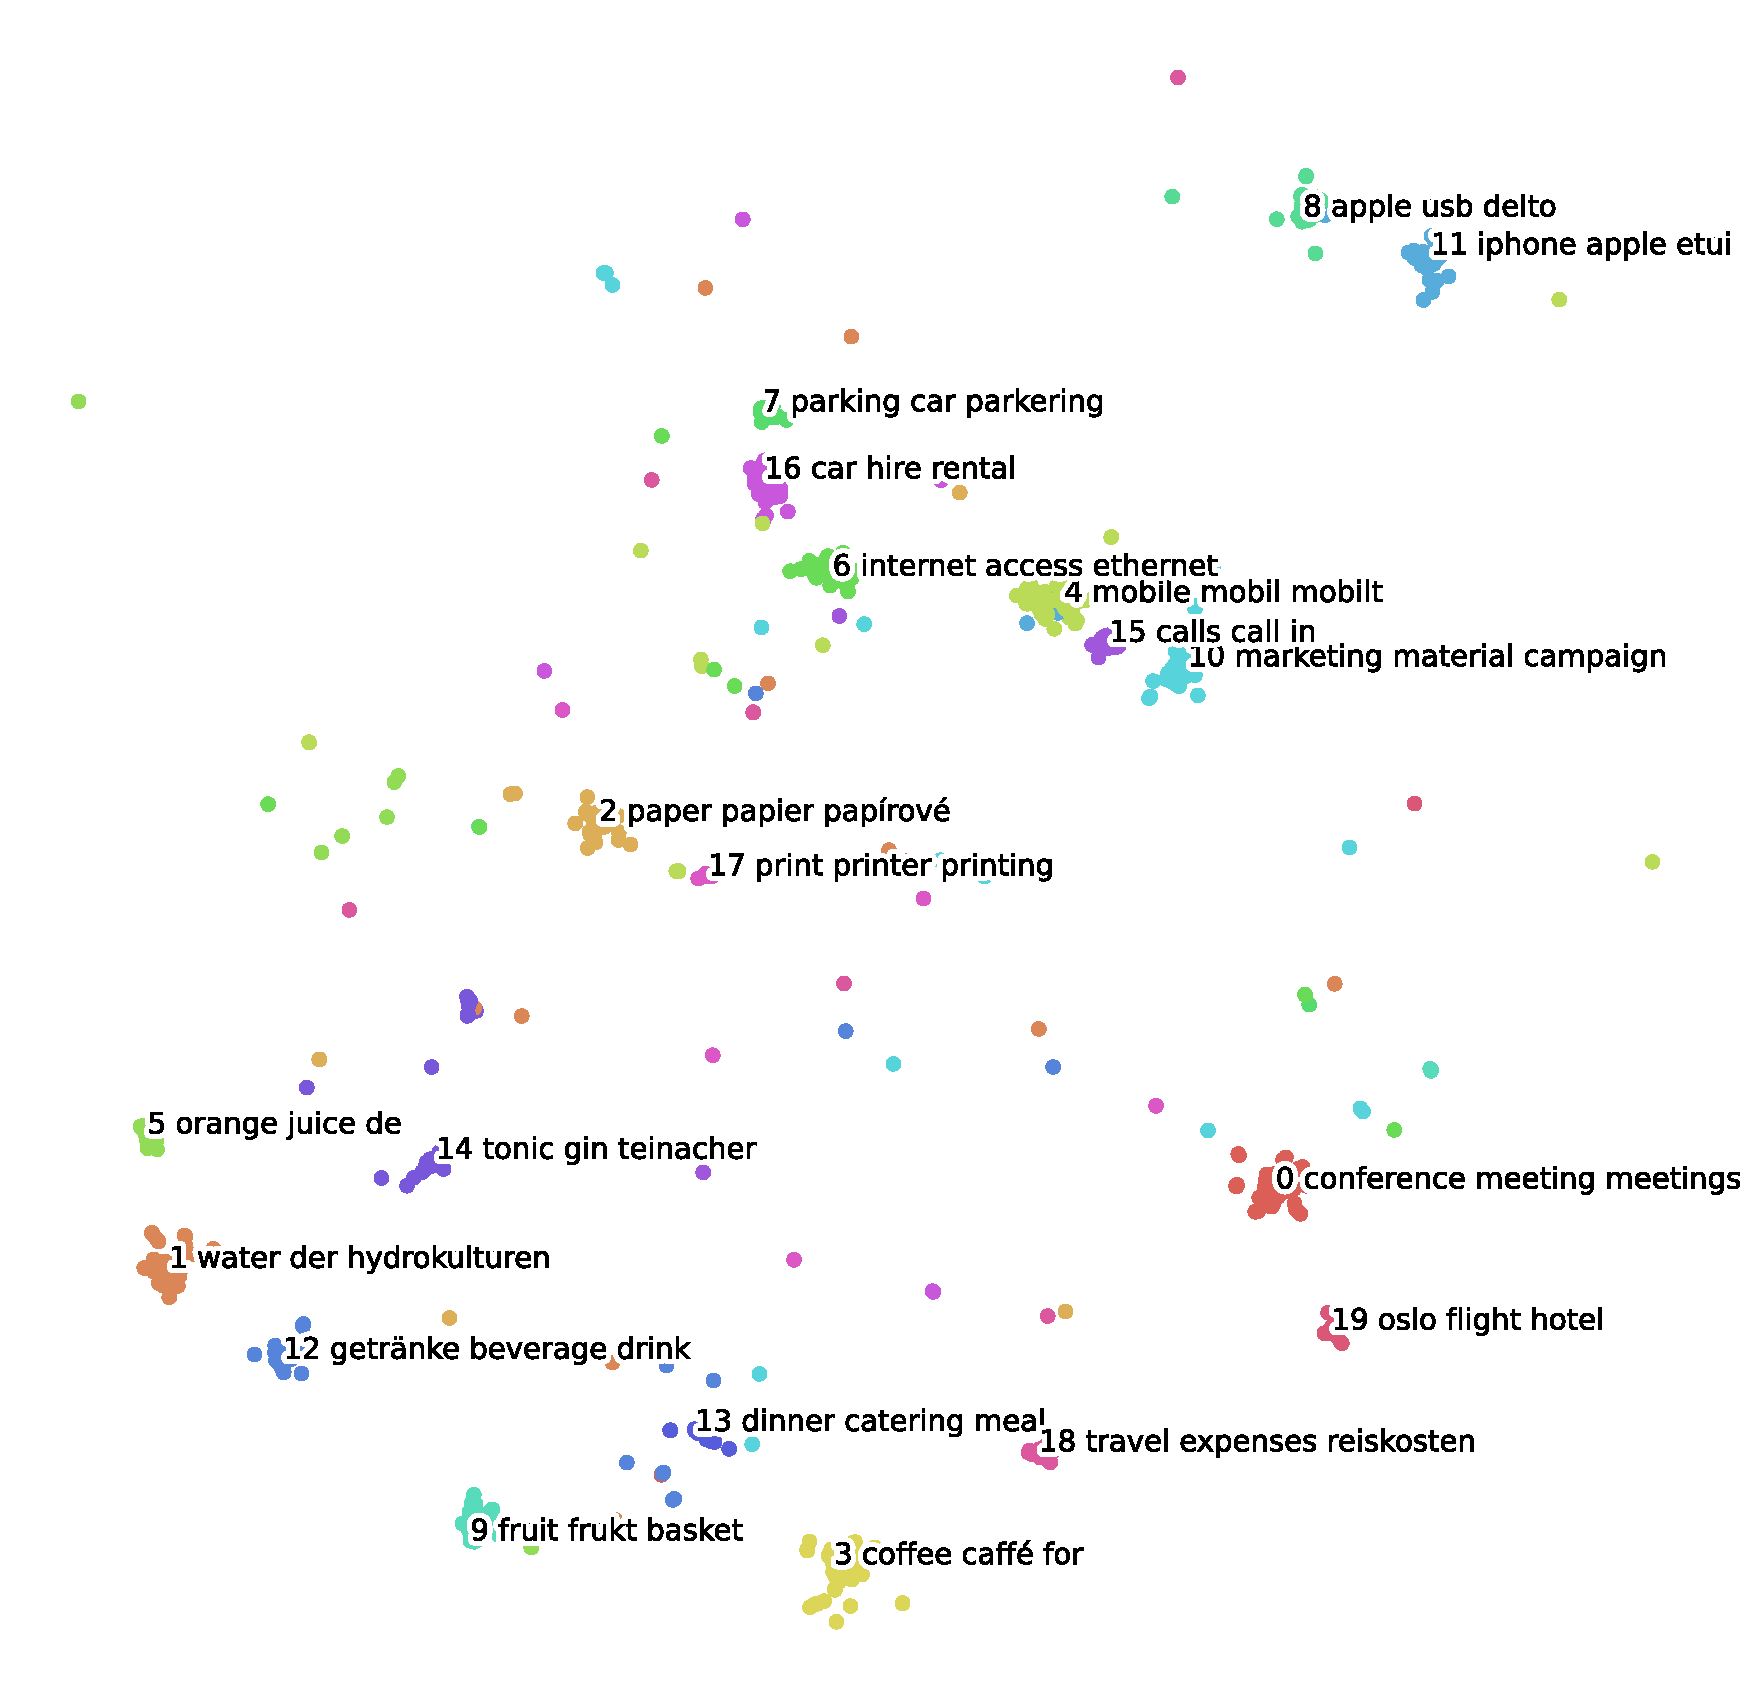
\includegraphics[width=\textwidth]{Bilder/models/topics.pdf}
	\caption{Selected Clusters and their Topics}
	\label{fig:topics}
\end{figure}

The chart \ref{fig:topics} seems to contain many outliers which are far away from their cluster. But, the outliers only appear to be so many, since the clusters are very dense. The chart contains more than 9000 data points, and most of them are so close to each other in one cluster, that they are indistinguishable from another.

What is striking about the clusters is the formation of areas where not only documents in one cluster are similar, but clusters are similar to each other. For example, clusters 5, 14, 1, and 12 form one area about drinking. Also, the four clusters are very close to 9 and 13. What too can be inferred is, that meals are connected with conferences through travel expenses. Additionally, these clusters are very far away from 8 and 11, which contain invoices on hardware. 

One proof, that the model captures the semantics of each word, is that the documents containing 'apple' (cluster 8, 11) are far away from the fruit basket cluster (9). The model understands, how in specific contexts 'Apple' stands for the brand and not the fruit.

Also in the north-western region of the chart, a cluster of clusters about services has formed. Although, a shorter distance between car renting (cluster 7, 16) and business travel (0, 18, 19) would be more understandable.
